% 2026 年全国大学生数学建模竞赛 C 题论文
% 正式提交电子版使用 withoutpreface；如需检查封面，可改为 \documentclass{cumcmthesis}。
\documentclass[withoutpreface,bwprint]{cumcmthesis}

\usepackage{cumcm2026}

% 图片统一存放在 src/figure；在线编译时保持 src/tex 与 src/figure 的相对位置。
\graphicspath{{../figure/}}

% ==================== 论文与队伍信息 ====================
\title{微网与外部电网电力调控策略}
\tihao{C}
\baominghao{待填写}
\schoolname{待填写}
\membera{cmx}
\memberb{xtc}
\memberc{lcy}
\supervisor{待填写}
\yearinput{2026}
\monthinput{9}
\dayinput{待填写}
% ========================================================

\begin{document}

\maketitle

\begin{abstract}
% TODO：概述问题背景、主要模型、求解方法、关键结果和结论。

\keywords{微网调度\quad 储能系统\quad 滚动优化\quad 强化学习\quad 不确定性}
\end{abstract}

% 竞赛论文通常不需要目录，写作阶段如需检查结构可临时取消下一行注释。
% \tableofcontents
% \newpage

\section{问题重述}

题目研究含光伏发电、储能设备和外部电网的并网型微网。微网需要在满足小区负荷的
前提下，根据电价、负荷、光伏功率和储能状态制定购电及充放电策略，以降低购电费用。
四个问题逐步增加实际运行中的不确定性：问题一要求在给定单日电价、负荷和光伏预测
的条件下求确定性最优调度；问题二需要利用历史数据制定日前计划，并承担预测偏差导致
的紧急购电费用；问题三允许在日内获得新的光伏预报后调整计划；问题四进一步考虑实时
波动电价。本文首先建立统一的能量平衡和储能状态模型，再分别处理确定性调度、预测误差、
滚动修正和电价波动。

\section{问题分析}

\subsection{问题一分析}

问题一中的电价、负荷和光伏预测均已知，且题目要求储能在 0:00 与 24:00 的储电量
相同。因此该问题本质上是具有跨时段状态耦合的确定性经济调度问题。各时段的购电量、
充电量和放电量为连续变量，购电费用与购电量线性相关，能量平衡、储能状态转移及容量
约束也均为线性关系，故可建立线性规划模型\cite{parisio2014}。其关键在于统一功率与电量的单位、正确放置
充放电效率，并通过周期边界条件避免模型在日末无偿释放剩余电能。在线性规划取得最低
购电费后，再最小化充放电总量，可以消除不影响费用的无意义循环充放电解。

\subsection{问题二分析}

% TODO：预测误差、储能安全余量和紧急购电。

\subsection{问题三分析}

% TODO：多时刻光伏预测、滚动优化和购电计划调整。

\subsection{问题四分析}

% TODO：波动电价下对问题二和问题三的扩展。

\section{模型假设}

\begin{enumerate}
  \item 附件给出的十分钟时刻功率代表对应十分钟时段内的平均功率，时段电量按平均
  功率乘以 $1/6$ 小时计算。该处理与附件的时间分辨率一致。
  \item 问题一中给定的电价、负荷和光伏预测在调度日前已知，并按题意视为逐日重复；
  不额外引入预测误差。
  \item 微网只能从外网购电，不能向外网售电。光伏电量优先供负荷或为储能充电，仍
  无法消纳的部分作为弃光量处理。
  \item 充电量和放电量均定义在交流母线侧，充、放电单向效率均为常数 $0.9$，故完整
  充放电循环的往返效率为 $0.9\times0.9=0.81$。效率仅计入储能状态方程，不重复计入
  母线能量平衡。
  \item 除储能充放电损耗外，忽略微网内部线路损耗、储能自放电、温度效应和功率爬坡
  过程。问题一只有一天且题目未给出相应参数，该简化可以避免引入缺乏依据的经验常数。
  \item 问题一暂不计电池寿命衰减成本。为排除线性规划的退化解，在最低购电费不变的
  条件下，以充放电总量最小作为第二级优化目标。
  \item 储能以 24 小时为一个运行周期，0:00 和 24:00 的储电量均为
  \SI{6000}{kWh}。附件中标记为 ``0:00+1'' 的周期数据在计算时旋转到序列首端，求解后
  再按结果模板的原顺序写回。
\end{enumerate}

\section{符号说明}

\begin{table}[H]
  \centering
  \caption{主要符号说明}
  \label{tab:symbols}
  \begin{tabularx}{\textwidth}{C{0.18\textwidth} L L}
    \toprule
    符号 & 含义 & 单位 \\
    \midrule
    $t$ & 十分钟决策时段索引 & -- \\
    $p_t$ & 时段 $t$ 的外网电价 & 元/kWh \\
    $L_t$ & 时段 $t$ 的小区负荷功率 & \si{kW} \\
    $P_t^{\mathrm{pv}}$ & 时段 $t$ 的光伏预测功率 & \si{kW} \\
    $g_t$ & 外部电网计划购电量 & \si{kWh} \\
    $c_t$ & 储能充电量 & \si{kWh} \\
    $d_t$ & 储能放电量 & \si{kWh} \\
    $e_t$ & 储能系统的储电量 & \si{kWh} \\
    $w_t$ & 无法消纳的弃光量 & \si{kWh} \\
    $\eta_c,\eta_d$ & 储能充电效率和放电效率 & -- \\
    $\Delta t$ & 单个决策时段的长度 & \si{h} \\
    \bottomrule
  \end{tabularx}
\end{table}

\section{数据预处理与预测方法}

\subsection{时间索引与单位换算}

一天被划分为 $T=144$ 个十分钟时段，记 $t=0,1,\ldots,T-1$，时间步长为
\begin{equation}
  \Delta t=\frac{10}{60}=\frac{1}{6}\ \mathrm{h}.
\end{equation}
附件中的负荷和光伏均为功率，而优化变量及结果文件使用电量；储能分析中必须明确区分
功率容量和能量容量\cite{nrel2022}。因此将输入转换为
\begin{equation}
  l_t=L_t\Delta t,\qquad v_t=P_t^{\mathrm{pv}}\Delta t.
\end{equation}
由此得到单时段最大充电量和放电量
\begin{equation}
  \bar c=\bar d=\SI{5000}{kW}\times\frac{1}{6}\ \mathrm{h}
  =\SI{833.3333}{kWh}.
\end{equation}

附件 1 与结果模板的时刻从 0:10 排列至第二天 0:00。为使初始状态严格对应题目
指定的 0:00，将 ``0:00+1'' 视作周期中的 0:00 并旋转到计算序列开头，形成
$0{:}00,0{:}10,\ldots,23{:}50$ 的状态递推顺序。由于问题一的数据和策略按日重复，
这种循环移位不改变目标函数和可行域，求解后再按模板顺序还原即可。

图~\ref{fig:q1-input} 展示了问题一的输入数据。光伏功率在中午附近超过负荷，而
电价在早晚存在明显峰谷，这为储能进行跨时段能量转移提供了空间。

\begin{figure}[H]
  \centering
  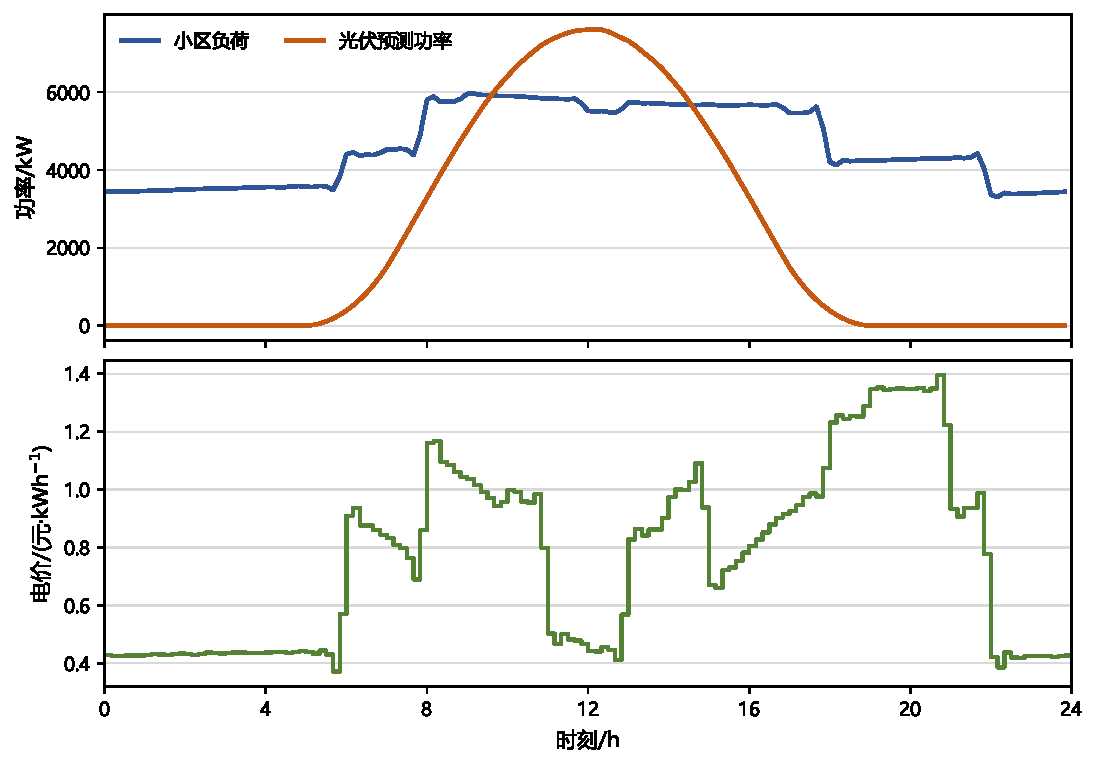
\includegraphics[width=0.92\textwidth]{q1_input_profile.pdf}
  \caption{问题一的负荷、光伏预测功率与分时电价}
  \label{fig:q1-input}
\end{figure}

\subsection{负荷与光伏预测}

% TODO：说明因果数据划分、预测模型和误差评价。

\subsection{电价数据处理}

% TODO：说明固定电价与波动电价的处理方式。

\section{问题一的确定性优化模型}

\subsection{模型建立}

令 $g_t,c_t,d_t,w_t$ 分别表示时段 $t$ 的计划购电量、母线侧充电量、母线侧
放电量和弃光量，$e_t$ 表示时段 $t$ 开始时储能内部的储电量。问题一的目标是使
全天购电费用最小：
\begin{equation}
  \min C=\sum_{t=0}^{T-1}p_tg_t.
  \label{eq:q1-objective}
\end{equation}

每个时段内，外网购电、光伏发电和储能放电共同满足负荷、储能充电及弃光需求，故有
\begin{equation}
  g_t+v_t+d_t=l_t+c_t+w_t,
  \qquad t=0,1,\ldots,T-1.
  \label{eq:q1-balance}
\end{equation}
由于 $c_t$ 和 $d_t$ 均在交流母线侧计量，储能状态转移方程为
\begin{equation}
  e_{t+1}=e_t+\eta_c c_t-\frac{d_t}{\eta_d},
  \qquad \eta_c=\eta_d=0.9.
  \label{eq:q1-soc}
\end{equation}
该效率处理与储能调度研究中常用的离散 SOC 方程一致\cite{gorman2024}。容量、功率和
弃光约束分别为
\begin{align}
  \SI{1200}{kWh}&\le e_t\le\SI{10800}{kWh}, \label{eq:q1-soc-bound}\\
  0&\le c_t,d_t\le\SI{833.3333}{kWh}, \label{eq:q1-power-bound}\\
  g_t&\ge 0,\qquad 0\le w_t\le v_t. \label{eq:q1-flow-bound}
\end{align}
其中 $g_t\ge0$ 表示不允许向外网反向售电。题目要求的周期边界条件写为
\begin{equation}
  e_0=e_T=\SI{6000}{kWh}.
  \label{eq:q1-terminal}
\end{equation}
式~\eqref{eq:q1-terminal} 消除了单日优化中的末端效应，使模型不能通过在最后时段
耗尽储能获得一次性的虚假收益。

\subsection{求解方法}

式~\eqref{eq:q1-objective}--\eqref{eq:q1-terminal} 构成标准线性规划，可使用成熟的
内点法或单法稳定求解\cite{boyd2004}。本文使用 SciPy 的 \texttt{linprog} 接口调用
HiGHS 求解器\cite{scipy2020}。为避免最优面上出现不增加购电费、但同时充放电的退化解，
采用两阶段字典序优化：第一阶段求得最低购电费 $C^*$；第二阶段增加约束 $C=C^*$，并求解
\begin{equation}
  \min \sum_{t=0}^{T-1}(c_t+d_t).
  \label{eq:q1-tiebreak}
\end{equation}
第二阶段不会改变经济最优值，只在等价最优解中选择储能动作最少的方案。求解后逐时段
检查式~\eqref{eq:q1-balance} 和式~\eqref{eq:q1-soc} 的残差，并检查 SOC、功率、非负性、
首末状态和充放电互斥性。完整程序见支撑材料 \texttt{src/py/question1.py}。

\subsection{结果与分析}

表~\ref{tab:q1-purchase} 给出题目指定时段的计划购电量。全天计划购电量为
\SI{59482.6990}{kWh}，相应购电费为 \num{35126.8486} 元。

\begin{table}[H]
  \centering
  \caption{问题一指定时段的计划购电量}
  \label{tab:q1-purchase}
  \begin{tabular}{cccccc}
    \toprule
    时间段 & 购电量/kWh & 时间段 & 购电量/kWh & 时间段 & 购电量/kWh \\
    \midrule
    10:00--10:10 & 0.0000 & 12:00--12:10 & 486.4029 & 14:00--14:10 & 0.0000 \\
    16:00--16:10 & 394.9315 & 18:00--18:10 & 636.9826 & 20:00--20:10 & 0.0000 \\
    \bottomrule
  \end{tabular}
\end{table}

表~\ref{tab:q1-storage} 给出六个四小时时段的充放电量。全天累计充电量为
\SI{20740.6661}{kWh}，累计放电量为 \SI{16799.9396}{kWh}，二者之比恰为
$0.81$，与周期边界下的往返效率 $\eta_c\eta_d=0.81$ 一致。

\begin{table}[H]
  \centering
  \caption{问题一储能设备分时段充放电结果}
  \label{tab:q1-storage}
  \begin{tabular}{ccccc}
    \toprule
    时间段 & 充电量/kWh & 放电量/kWh & 时刻 & 储电量/kWh \\
    \midrule
    0:00--4:00   & 4500.0000 & 0.0000    & 0:00  & 6000.0000 \\
    4:00--8:00   & 833.3333  & 5947.4198 & 24:00 & 6000.0000 \\
    8:00--12:00  & 3954.6310 & 2121.4184 & -- & -- \\
    12:00--16:00 & 6119.3685 & 91.1014   & -- & -- \\
    16:00--20:00 & 0.0000    & 5068.6869 & -- & -- \\
    20:00--24:00 & 5333.3333 & 3571.3132 & -- & -- \\
    \bottomrule
  \end{tabular}
\end{table}

图~\ref{fig:q1-schedule} 表明，策略在低价时段集中购电并充电，在光伏出力较高时减少
外网购电，在晚间高价时段通过放电削减购电。最低电价出现在 5:40--5:50，为
\num{0.3713} 元/kWh；最高电价出现在 20:40--20:50，为 \num{1.3952} 元/kWh。
储能的充放电方向与价格变化总体一致，但仍受光伏剩余量、负荷和功率上限共同约束。

\begin{figure}[H]
  \centering
  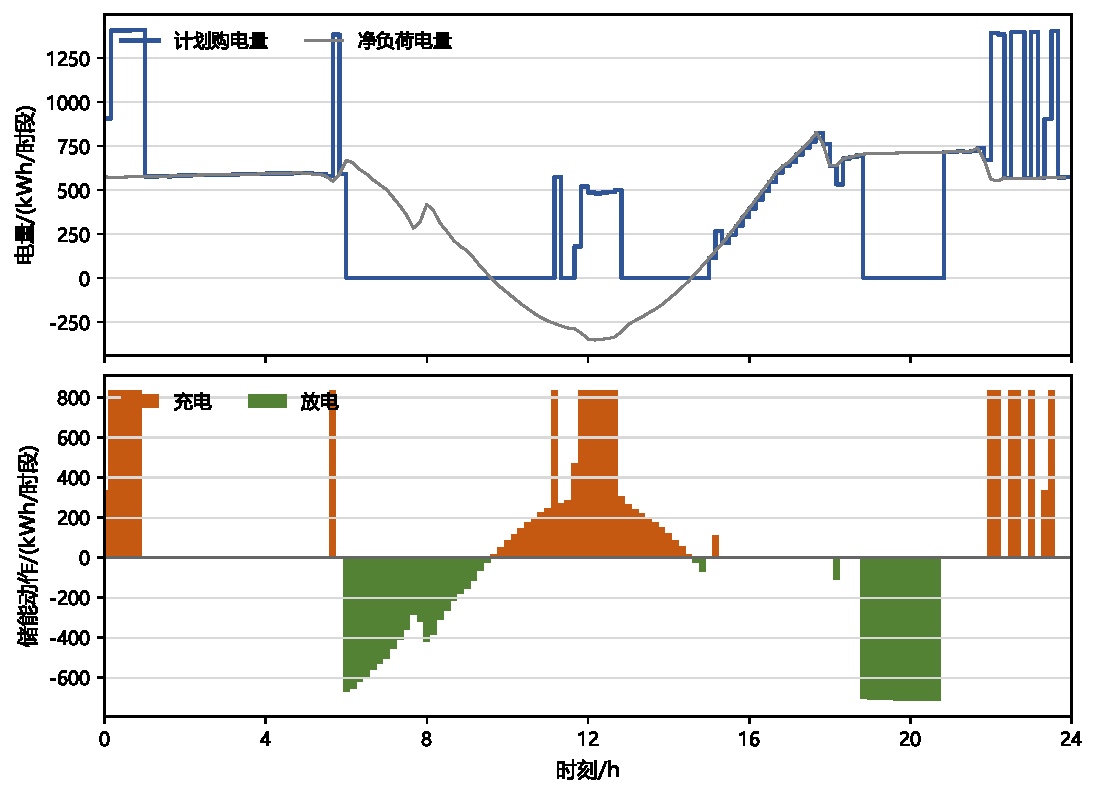
\includegraphics[width=0.92\textwidth]{q1_optimal_schedule.pdf}
  \caption{问题一的最优购电与储能调度策略}
  \label{fig:q1-schedule}
\end{figure}

由图~\ref{fig:q1-soc} 可见，储电量始终位于 \SIrange{1200}{10800}{kWh}，且在部分
时段达到上下边界，说明给定储能容量得到充分利用；0:00 和 24:00 均回到
\SI{6000}{kWh}。模型的最大能量平衡残差为 $1.89\times10^{-11}$ kWh，最大 SOC
递推残差为 $9.09\times10^{-13}$ kWh，且没有出现同时充放电。

\begin{figure}[H]
  \centering
  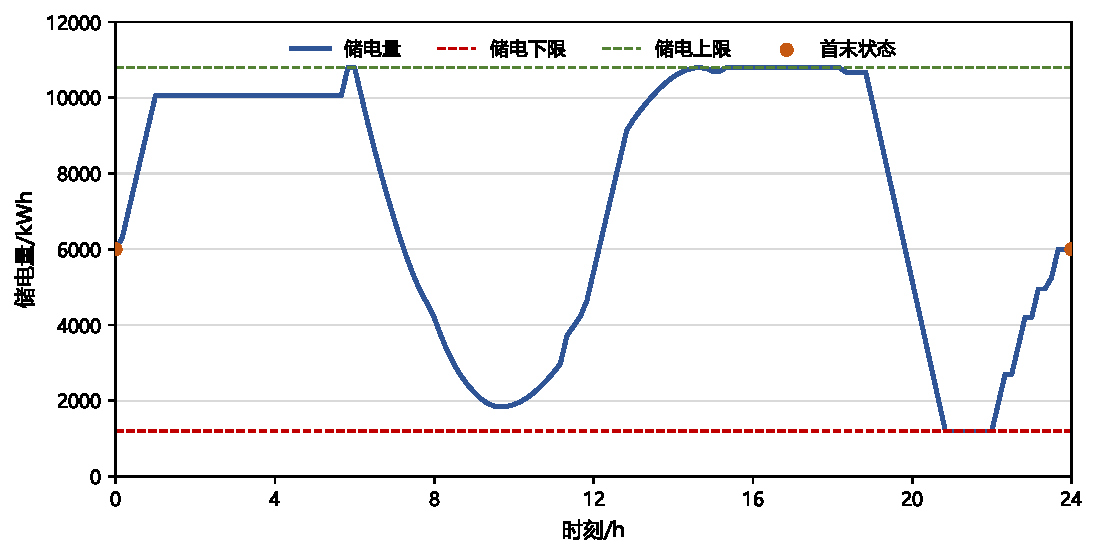
\includegraphics[width=0.92\textwidth]{q1_soc.pdf}
  \caption{问题一储能设备的储电量变化}
  \label{fig:q1-soc}
\end{figure}

为评价储能调度的经济作用，构造“不使用储能、光伏优先供负荷”的基准策略。该策略的
购电费为 \num{48052.0466} 元，而优化策略节省 \num{12925.1980} 元，降幅为
\SI{26.90}{\percent}。优化结果的弃光量为 0，光伏消纳率达到 \SI{100}{\percent}。
这说明在给定数据下，储能不仅通过峰谷价差降低费用，也吸收了中午光伏剩余电量。
完整的 144 个时段计划已写入 \texttt{src/附件5/result1.xlsx}。

\section{问题二的预测误差调度模型}

\subsection{日前计划与紧急购电机制}

% TODO：定义计划购电、实际供需缺口和五倍价格紧急购电。

\subsection{优化与控制策略}

% TODO：说明预测模型、基准优化器以及强化学习修正策略。

\subsection{结果与分析}

% TODO：填写 result2.xlsx，统计正常购电、紧急购电和总费用。

\section{问题三的滚动调整模型}

\subsection{多时刻光伏预测更新}

% TODO：说明 0、6、12、18 点预测的对齐和十分钟插值。

\subsection{滚动优化与调整费用}

% TODO：说明向上调整、向下调整和紧急购电的费用口径。

\subsection{预测更新频率分析}

% TODO：比较不同更新间隔的成本、收益和计算时间。

\subsection{结果与分析}

% TODO：填写 result3.xlsx，并分析滚动调整的价值。

\section{问题四的波动电价模型}

\subsection{波动电价下的问题二}

% TODO：生成 result4-2.xlsx，并与固定电价结果比较。

\subsection{波动电价下的问题三}

% TODO：生成 result4-3.xlsx，并与固定电价结果比较。

\subsection{结果对比}

% TODO：讨论价格预测、负荷预测和光伏预测共同不确定时的策略表现。

\section{模型评价与敏感性分析}

\subsection{方法对比与消融实验}

% TODO：比较规则策略、线性规划、滚动优化、纯强化学习和混合策略。

\subsection{敏感性分析}

% TODO：分析预测误差、储能容量、功率、效率和初始电量的影响。

\subsection{模型优缺点}

% TODO：总结模型的适用条件、优势和局限。

\section{结论}

% TODO：逐问总结主要结论，并给出可执行的微网调度建议。

% 2026 年竞赛要求在参考文献之前声明 AI 工具使用情况。
\CumcmAIUsed{资料整理、思路讨论、代码调试和语言润色}

\begin{thebibliography}{99}
  \bibitem{nrel2022} P. Joshi and C. Gokhale-Welch. Fundamentals of Energy
  Storage[R]. Golden: National Renewable Energy Laboratory, 2022.

  \bibitem{gorman2024} W. Gorman, G. Barbose, C. Miller, et al. Evaluating the
  potential for solar-plus-storage backup power in the United States as homes
  integrate efficient, flexible, and electrified energy technologies[J].
  Energy, 2024, 304: 132180.

  \bibitem{parisio2014} A. Parisio, E. Rikos, G. Tzamalis, et al. Use of model
  predictive control for experimental microgrid optimization[J]. Applied Energy,
  2014, 115: 37--46.

  \bibitem{boyd2004} S. Boyd and L. Vandenberghe. Convex Optimization[M].
  Cambridge: Cambridge University Press, 2004.

  \bibitem{scipy2020} P. Virtanen, R. Gommers, T. E. Oliphant, et al. SciPy 1.0:
  Fundamental algorithms for scientific computing in Python[J]. Nature Methods,
  2020, 17: 261--272.
\end{thebibliography}

\newpage
\begin{appendices}

\section{主要程序代码}

% TODO：放置关键算法代码或说明完整代码所在的支撑材料文件。

\section{补充结果}

% TODO：放置正文中不便展开的表格、图形和验证结果。

\section{AI 工具使用详情索引}

% TODO：按照竞赛要求另行生成“AI工具使用详情.pdf”，此处列出对应材料索引。

\end{appendices}

\end{document}
